26. \begin{figure}[ht!]
\center{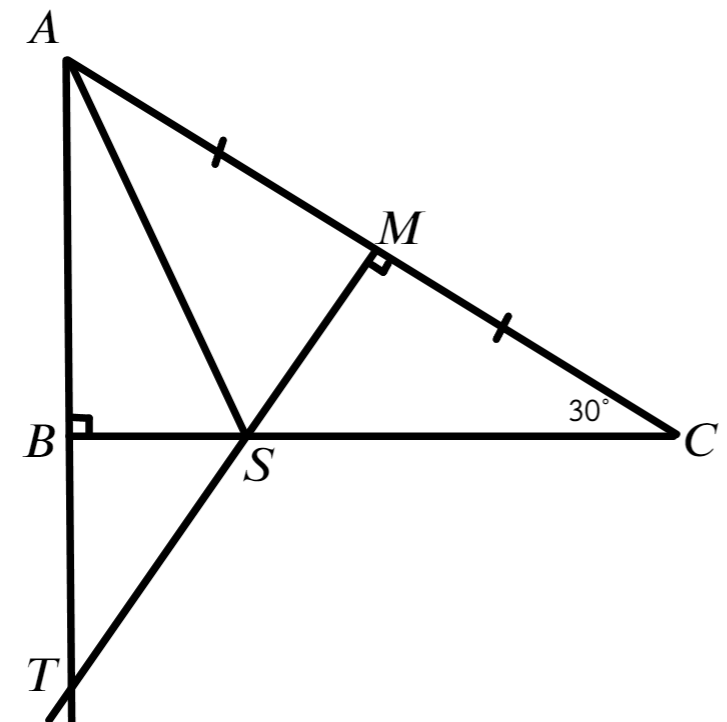
\includegraphics[scale=0.35]{g26.png}}
\end{figure}\\
$\angle C=90^\circ-\angle A=90^\circ-60^\circ=30^\circ.$ Пусть $MT$ пересекает сторону $BC$ в точке $S.$ Так как в треугольнике $ASC$ высота совпала с медианой, он является равнобедренным, поэтому $\angle SAC=\angle C=30^\circ.$ Тогда $\angle BAS=\angle A-\angle SAC=60^\circ-30^\circ=30^\circ.$ В прямоугольных треугольниках $SAM$ и $SCM$ катет $MS$ лежит напротив угла в $30^\circ,$ а значит $AS=SC=2MS.$ В прямоугольном треугольнике $ABS$ катет $BS$ лежит напротив угла
в $30^\circ,$ а значит $BS=AS:2=2MS:2=MS.$ Таким образом, $BC=BS+SC=MS+2MS=3MS=3$см, откуда $MS=3:3=1$см. Из треугольника $TAM$ найдём $\angle ATM=90^\circ-60^\circ=30^\circ.$ В прямоугольном треугольнике $TBS$ катет $BS$ лежит напротив угла в $30^\circ,$ значит $ST=2BS=2\cdot1=2$см. Таким образом, $MT=MS+ST=1+2=3$см.\\
